%************************************************
\chapter{System Model}\label{ch:model} 
%************************************************
%VWrite about the model and how it was built. 3D model of house was provided... Used software \texttt{Modelica}...
%Demonstate how model (acturately) predicts how the residential home behaves in real life to certain degree... Compare simulation to real life restults... Explain inaccuracies... which assumptions lead to these...
% Thermodynamic model, assumptions, constraints, design point conditions etc. 
% Equations 
% economic and ecological models. 

\begin{flushright}{\slshape
    The purpose of models is not to fit the data, but to sharpen the question} \\ \medskip
    --- Samuel Karlin
\end{flushright}

\section{Location}
The reference house that the building model is based off of a hipped dormer, two-storey residential house located in Belturbet, Cavan, a small town close to the Republic of Ireland and Northern Ireland border, about 125 kilometres from Dublin. The reference house lies at an elevation of 80 metres and is Easterly facing. The dwelling is located in a residential estate, and is thus classified as being located in an urban environment.

\section{Form and Fabric}
The reference model has a floor area of 160 square metres, 93 square metres of which are downstairs, i.e., ``exterior floor'', a gross roof area of 173 square metres and a total external wall surface area of 139 square metrse. There are 21 exterior windows of varying sizes in total and thirteen rooms, seven downstairs and six upstairs. The ceiling height is a uniform 2.5 metres throughout the model. All rooms except for one were considered to be unconditioned, the exception being a very small box room on the ground floor which was interpreted to be a utility room of sorts. The void zones were also unconditioned. The building model geometry and thermal properties were created during previous works by \citeauthor{keogh_technical_2022}. A floor plan schematic can be seen in \cref{fig:floorplan}, showing the ground floor and first floor room layouts and windows. A 3D rendered model of the house can be seen in \cref{fig:3dmodel}. All model data is contained in a \texttt{.idf} file, an input data file interpretable by \texttt{EnergyPlus}. This file contains data about the geometry of the building, envelope construction, thermal and physical properties of the constructions, building and occupancy schedules, internal gains, outside air infiltration to void zones and various other data regarding the simulation process e.g., timestep. 

\begin{figure}[htb]
    \centering
    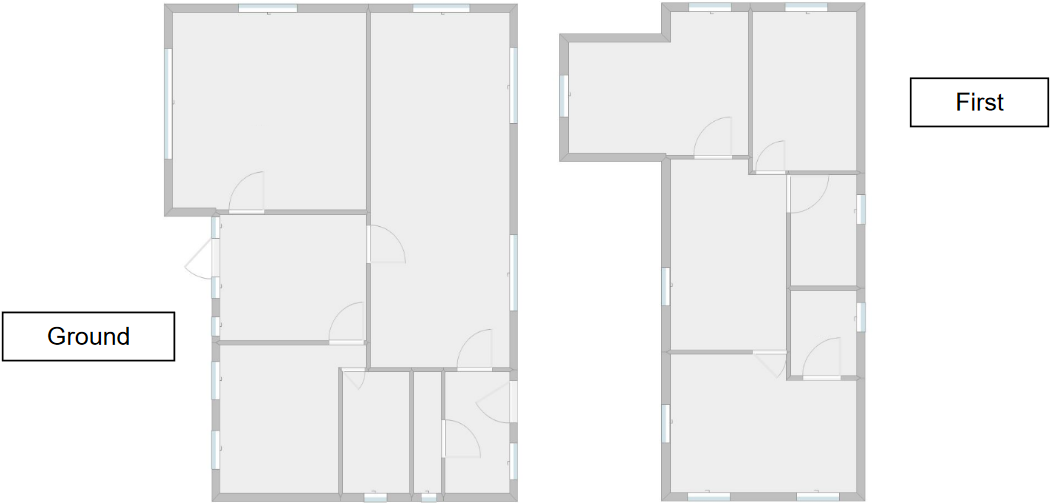
\includegraphics[width=0.75\linewidth]{dwellingFloorPlan}
    \caption{Dwelling Floor Plan}
    \label{fig:floorplan}
\end{figure}

\begin{figure}[htb]
    \centering
    %\includegraphics[width=0.7\linewidth]{3dmodel}
    \includegraphics[width=0.7\linewidth]{example-image-a}
    \caption[3D Model of Reference Building]{3D Model of Reference Building, rendered in SketchUp and the XXX plugin}
    \label{fig:3dmodel}
\end{figure}


\subsection{Thermal Properties of Constructions}

\begin{table}[htb]
    \footnotesize
    \centering
    \caption{Summary of U-Values}
    \label{tbl:uvalues}  
    \begin{tabular}{lccccc}\toprule
        \multicolumn{1}{c}{\multirow{2}{*}{\begin{tabular}[c]{@{}c@{}}Building \\ Model\end{tabular}}} & \multicolumn{4}{c}{\begin{tabular}[c]{@{}c@{}}U-Value\\ {[}W/m2-K{]}\end{tabular}} & \multirow{2}{*}{\begin{tabular}[c]{@{}c@{}}Infiltration\\ Rate\\ ACH\end{tabular}} \\ \cmidrule(lr){2-5}
        \multicolumn{1}{c}{} & \begin{tabular}[c]{@{}c@{}}Exterior\\ Wall\end{tabular} & \begin{tabular}[c]{@{}c@{}}Pitched\\ Roof\end{tabular} & \begin{tabular}[c]{@{}c@{}}Exterior\\ Floor\end{tabular} & \begin{tabular}[c]{@{}c@{}}Exterior\\ Glazing\end{tabular} &  \\ \midrule
        \begin{tabular}[c]{@{}l@{}}Minimal\\ Retrofit\end{tabular} & 0.31 & 0.16 & 0.25 & 2.15 & 0.8 \\
        \begin{tabular}[c]{@{}l@{}}Deep \\ Retrofit\end{tabular} & 0.18 & 0.16 & 0.18 & 1.39 & 0.5 \\ \bottomrule   
    \end{tabular}
\end{table}

\subsubsection{Minimal Retrofit Model}
\cref{tbl:extwallconst} details the specifications of the exterior wall construction for the minimal retrofit model, from outside to inside. 
\begin{table}[htb]
    \footnotesize
    \centering
    \caption{Exterior Wall Construction}
    \label{tbl:extwallconst}
    \begin{tabular}{lcccc}
        \toprule
        Layer        & \multicolumn{1}{c}{\begin{tabular}[c]{@{}c@{}}Thickness \\ {[}m{]}\end{tabular}} & \multicolumn{1}{c}{\begin{tabular}[c]{@{}c@{}}Density \\ {[}\unit{\kilogram\per\cubic\meter}{]}\end{tabular}} & \multicolumn{1}{c}{\begin{tabular}[c]{@{}c@{}}Heat Capacity \\  {[}\unit{\joule\per\kilogram\per\kelvin}{]}\end{tabular}}  & \multicolumn{1}{c}{\begin{tabular}[c]{@{}c@{}}Conductivity \\   {[}\unit{\watt\per\meter\per\kelvin}{]}\end{tabular}} \\ \midrule
        Rainscreen   & 0.01              & 7824                & 500                        & 30                       \\
        Insulation   & 0.085             & 43                  & 1210                       & 0.03                     \\
        Air Cavity      & 0.15              & $-$                  & $-$                      &  $-$                  \\
        Gypsum board & 0.019             & 800                 & 1090                       & 0.16                     \\
        \bottomrule
    \end{tabular}
\end{table}

\cref{tbl:extfloorconst} details the specifications of the exterior floor construction for the minimal retrofit model, from top to bottom. The exterior floor is the floor which lays on top of the foundations and therefore conducts heat from the inside of the house to the ground. It consists of concrete at the bottom, insulation board, an air cavity and floor tiles on top.

\begin{table}[htb]
    \footnotesize
    \centering
    \caption{Exterior Floor Construction}
    \label{tbl:extfloorconst}
    \begin{tabular}{lcccc}
        \toprule
        Layer        & \multicolumn{1}{c}{\begin{tabular}[c]{@{}c@{}}Thickness \\ {[}m{]}\end{tabular}} & \multicolumn{1}{c}{\begin{tabular}[c]{@{}c@{}}Density \\ {[}\unit{\kilogram\per\cubic\meter}{]}\end{tabular}} & \multicolumn{1}{c}{\begin{tabular}[c]{@{}c@{}}Heat Capacity \\  {[}\unit{\joule\per\kilogram\per\kelvin}{]}\end{tabular}}  & \multicolumn{1}{c}{\begin{tabular}[c]{@{}c@{}}Conductivity \\   {[}\unit{\watt\per\meter\per\kelvin}{]}\end{tabular}} \\ \midrule
        Acoustic Tile   & 0.0191            & 368                 & 590                        & 0.06                     \\
        Air Cavity      & 0.15              & $-$                  & $-$                      &  $-$                  \\
        Insulation      & 0.085             & 43                  & 1210                       & 0.03                     \\
        Concrete        & 0.1016             & 1280                 & 840                       & 0.53                     \\
        \bottomrule
    \end{tabular}
\end{table}


\cref{tbl:pitchroofconst} details the specifications of the pitched roof construction for the minimal retrofit model, from outside to inside. This construction is applied to the bulk of the roof and consists of clay tile, an air cavity, insulation board and then plasterboard. This construction remains the same across the minimal retrofit and deep retrofit models.

\begin{table}[htb]
    \footnotesize
    \centering
    \caption{Pitched Roof Construction}
    \label{tbl:pitchroofconst}
    \begin{tabular}{lcccc}
        \toprule
        Layer        & \multicolumn{1}{c}{\begin{tabular}[c]{@{}c@{}}Thickness \\ {[}m{]}\end{tabular}} & \multicolumn{1}{c}{\begin{tabular}[c]{@{}c@{}}Density \\ {[}\unit{\kilogram\per\cubic\meter}{]}\end{tabular}} & \multicolumn{1}{c}{\begin{tabular}[c]{@{}c@{}}Heat Capacity \\  {[}\unit{\joule\per\kilogram\per\kelvin}{]}\end{tabular}}  & \multicolumn{1}{c}{\begin{tabular}[c]{@{}c@{}}Conductivity \\   {[}\unit{\watt\per\meter\per\kelvin}{]}\end{tabular}} \\ \midrule
        Clay Tile   & 0.025            & 1900                 & 800                        & 0.84                     \\
        Air Cavity      & 0.15              & $-$                  & $-$                      &  $-$                  \\
        Insulation      & 0.162            & 43                  & 1210                       & 0.03                     \\
        Gypsum board & 0.019             & 800                 & 1090                       & 0.16                     \\
        \bottomrule
    \end{tabular}
\end{table}

The dormer roof provides no insulation and is only in place to protect the inside spaces from wind and rain. This construction is shared between the minimal retrofit model and the deep retrofit model.
\begin{table}[htb]
    \footnotesize
    \centering
    \caption{Hipped Dormer Roof Construction}
    \label{tbl:dormerroofconst}
    \begin{tabular}{lcccc}
        \toprule
        Layer        & \multicolumn{1}{c}{\begin{tabular}[c]{@{}c@{}}Thickness \\ {[}m{]}\end{tabular}} & \multicolumn{1}{c}{\begin{tabular}[c]{@{}c@{}}Density \\ {[}\unit{\kilogram\per\cubic\meter}{]}\end{tabular}} & \multicolumn{1}{c}{\begin{tabular}[c]{@{}c@{}}Heat Capacity \\  {[}\unit{\joule\per\kilogram\per\kelvin}{]}\end{tabular}}  & \multicolumn{1}{c}{\begin{tabular}[c]{@{}c@{}}Conductivity \\   {[}\unit{\watt\per\meter\per\kelvin}{]}\end{tabular}} \\ \midrule
        Clay Tile   & 0.025            & 1900                 & 800                        & 0.84                     \\
        Air Cavity      & 0.15              & $-$                  & $-$                      &  $-$                  \\
        Roofing Felt      & 0.005            & 960                  & 837                      & 0.19                    \\
        \bottomrule
    \end{tabular}
\end{table}

\begin{table}[htb]
    \footnotesize
    \centering
    \caption{External Glazing Construction}
    \label{tbl:glazingconst}
    \begin{tabular}{lccc}
        \toprule
        Layer        & \multicolumn{1}{c}{\begin{tabular}[c]{@{}c@{}}Thickness \\ {[}m{]}\end{tabular}} & \multicolumn{1}{c}{\begin{tabular}[c]{@{}c@{}}Transmittance \\ {[}\unit{\kilogram\per\cubic\meter}{]}\end{tabular}}  & \multicolumn{1}{c}{\begin{tabular}[c]{@{}c@{}}Conductivity \\   {[}\unit{\watt\per\meter\per\kelvin}{]}\end{tabular}} \\ \midrule
        Inner Pane   & 0.003            & 0.783                 & 0.4                                         \\
        Argon Gas      & 0.20              & $-$                  & $-$                                   \\
        Outer Pane     & 0.003            & 0.783                  & 0.4                                    \\
        \bottomrule
    \end{tabular}
\end{table}

\subsubsection{Deep Retrofit Model}
During the deep retrofit process, the external wall, exposed floor and external glazing constructions are upgraded to conform to the Building Regulations Part L 2022. The infiltration rate was also decreased to 0.5 \ac{ACPH} due to leakiness being heavily reduced.

\begin{table}[htb]
    \footnotesize
    \centering
    \caption{External Glazing Construction (Deep Retrofit)}
    \label{tbl:deepglazingconst}
    \begin{tabular}{lccc}
        \toprule
        Layer        & \multicolumn{1}{c}{\begin{tabular}[c]{@{}c@{}}Thickness \\ {[}m{]}\end{tabular}} & \multicolumn{1}{c}{\begin{tabular}[c]{@{}c@{}}Transmittance \\ {[}\unit{\kilogram\per\cubic\meter}{]}\end{tabular}}  & \multicolumn{1}{c}{\begin{tabular}[c]{@{}c@{}}Conductivity \\   {[}\unit{\watt\per\meter\per\kelvin}{]}\end{tabular}} \\ \midrule
        Inner Pane   & 0.003            & 0.783                 & 0.4                                         \\
        Argon Gas      & 0.20              & $-$                  & $-$                                   \\
        Middle Pane   & 0.003            & 0.783                 & 0.4                                         \\
        Argon Gas      & 0.20              & $-$                  & $-$                                   \\
        Outer Pane     & 0.003            & 0.783                  & 0.4                                    \\
        \bottomrule
    \end{tabular}   
\end{table}

\begin{table}[htb]
    \footnotesize
    \centering
    \caption{Exterior Floor Construction}
    \label{tbl:deepextfloorconst}
    \begin{tabular}{lcccc}
        \toprule
        Layer        & \multicolumn{1}{c}{\begin{tabular}[c]{@{}c@{}}Thickness \\ {[}m{]}\end{tabular}} & \multicolumn{1}{c}{\begin{tabular}[c]{@{}c@{}}Density \\ {[}\unit{\kilogram\per\cubic\meter}{]}\end{tabular}} & \multicolumn{1}{c}{\begin{tabular}[c]{@{}c@{}}Heat Capacity \\  {[}\unit{\joule\per\kilogram\per\kelvin}{]}\end{tabular}}  & \multicolumn{1}{c}{\begin{tabular}[c]{@{}c@{}}Conductivity \\   {[}\unit{\watt\per\meter\per\kelvin}{]}\end{tabular}} \\ \midrule
        Acoustic Tile   & 0.0191            & 368                 & 590                        & 0.06                     \\
        Air Cavity      & 0.15              & $-$                  & $-$                      &  $-$                  \\
        Insulation      & 0.085             & 43                  & 1210                       & 0.03                     \\
        Concrete        & 0.1016             & 1280                 & 840                       & 0.53                     \\
        \bottomrule
    \end{tabular}
\end{table}

\begin{table}[htb]
    \footnotesize
    \centering
    \caption{Exterior Wall Construction}
    \label{tbl:deepextwallconst}
    \begin{tabular}{lcccc}
        \toprule
        Layer        & \multicolumn{1}{c}{\begin{tabular}[c]{@{}c@{}}Thickness \\ {[}m{]}\end{tabular}} & \multicolumn{1}{c}{\begin{tabular}[c]{@{}c@{}}Density \\ {[}\unit{\kilogram\per\cubic\meter}{]}\end{tabular}} & \multicolumn{1}{c}{\begin{tabular}[c]{@{}c@{}}Heat Capacity \\  {[}\unit{\joule\per\kilogram\per\kelvin}{]}\end{tabular}}  & \multicolumn{1}{c}{\begin{tabular}[c]{@{}c@{}}Conductivity \\   {[}\unit{\watt\per\meter\per\kelvin}{]}\end{tabular}} \\ \midrule
        Rainscreen   & 0.01              & 7824                & 500                        & 30                       \\
        Insulation   & 0.085             & 43                  & 1210                       & 0.03                     \\
        Air Cavity      & 0.15              & $-$                  & $-$                      &  $-$                  \\
        Gypsum board & 0.019             & 800                 & 1090                       & 0.16                     \\
        \bottomrule
    \end{tabular}
\end{table}



 

\section{Schedules, Equipment and Internal Gains}
Internal gains in the context of an energy building simulation of a residential home refers to the heat generated within the envelope by people, appliances, and lighting.

People generate heat through their activities and body heat, while appliances generate heat through their operation. Lighting generates heat due to the inefficiencies in converting electricity into light, and light ultimately being converted to heat energy.

In energy building simulation, internal gains are important to consider because they can significantly affect the energy balance of the building. If the internal gains are high, the building may require less heating, which can lead to energy savings. Conversely, if the internal gains are low, the building may require more heating, which can lead to increased energy consumption and costs. \cite{buttitta_high-temporal_2020}

Internal gains are typically modelled as a heat input to the building, which is then factored into the overall energy balance of the building. The magnitude of internal gains is typically calculated based on the number of occupants, the types and number of appliances, and the lighting levels in the building.

\subsection{Occupancy Gains}
The magnitude of these gains depends on factors such as the number of occupants, their activity levels, and the duration of their stay in the building. It was decided that a house of the size of the reference home was sized for a total of four persons. 

In order to accurately model occupancy gains in a building energy simulation, it is important to use typical occupancy profiles in conjunction with typical metabolic rates for different tasks. A typical occupancy profile is a representation of the number of occupants in the building over time, while a typical metabolic rate is a measure of the heat generated by a person due to their physical activity. Different tasks require different amounts of energy, and therefore result in different levels of heat generation. For example, a person sitting quietly may have a lower metabolic rate than someone performing strenuous physical activity.

\citeauthor{buttitta_high-temporal_2020} \cite{buttitta_high-temporal_2020} developed a stochastic occupancy model which generates hourly occupancy schedules for up to five different types of occupancy profiles of residential buildings for an entire year, based off of data gathered from London, UK. For this thesis, an occupancy profile was chosen which represented the largest share of the population, and two schedules were drawn, one for the weekdays and one for the weekends. These schedules depict the number of persons occupying the dwelling at each hour of the day, and are detailed in \cref{tbl:occupancysched}.

\begin{table}[htb]
    \centering
    \caption{Occupancy Schedules}
    \label{tbl:occupancysched}
    \begin{tabular}
        {lcr}
        \toprule
        1&1&1\\
        \bottomrule
    \end{tabular}
\end{table}

\citetitle{ashrae_ansiashrae_2010} \cite{ashrae_ansiashrae_2010} details the metabolic rate of people performing various tasks, given in Met units, as well as watts per square metre. An activity level schedule was quasi-arbitrarily assembled and is detailed in \cref{tbl:activitysched}.

\begin{table}[htb]
    \centering
    \caption{Activity Schedule}
    \label{tbl:activitysched}
    \begin{tabular}
        {lcr}
        \toprule
        1&1&1\\
        \bottomrule
    \end{tabular}
\end{table}

\subsection{Lighting}
In the past, internal gains from lighting used to be a significant contributor to the overall heat load of buildings. This was largely due to the widespread use of inefficient incandescent light bulbs, which generated a significant amount of heat as a byproduct of their operation. In fact, it was not uncommon for incandescent bulbs to emit more heat than light, resulting in a significant waste of energy and contributing to higher cooling loads in buildings.

However, with the gradual adoption of more efficient lighting technologies such as LED bulbs, internal gains from lighting have become much less of a concern. LED bulbs are significantly more efficient than incandescent bulbs, converting a higher percentage of their energy input into light rather than heat. This means that they generate far less waste heat, resulting in lower cooling loads and reduced energy consumption. \citefield{ISO17772}{shorttitle} presents lighting schedules and load density profiles for single family residential homes, and are reproduced in \cref{tbl:lightandequip}. 

\subsection{Plug Loads and Equipment}
Plug loads in a residential home refer to the energy consumed by appliances and devices that are plugged into electrical outlets, such as televisions, computers, and kitchen appliances. Equipment internal gains in a residential home refer to the heat generated by the operation of various equipment and appliances, such as refrigerators, ovens, and water heaters. This heat can contribute to the overall heat load of the home, particularly during periods of high use. \citefield{ISO17772}{shorttitle} gives details regarding standards for schedules and load density profiles for equipment gains and plug loads, and is reproduced in \cref{tbl:lightandequip}.

\begin{table}[htb]
    \centering
    \caption{Lighting, Plug Loads and Equipment Gains Schedules and Load Densities \cite{ISO17772}}
    \label{tbl:lightandequip}
    \begin{tabular}
        {lcr}
        \toprule
        2.07&1.92   &1\\
        \bottomrule
    \end{tabular}
\end{table}

\section{Climate}


\section{Load Profiles}